% Options for packages loaded elsewhere
\PassOptionsToPackage{unicode}{hyperref}
\PassOptionsToPackage{hyphens}{url}
%
\documentclass[
]{article}
\usepackage{amsmath,amssymb}
\usepackage{lmodern}
\usepackage{iftex}
\ifPDFTeX
  \usepackage[T1]{fontenc}
  \usepackage[utf8]{inputenc}
  \usepackage{textcomp} % provide euro and other symbols
\else % if luatex or xetex
  \usepackage{unicode-math}
  \defaultfontfeatures{Scale=MatchLowercase}
  \defaultfontfeatures[\rmfamily]{Ligatures=TeX,Scale=1}
  \setmainfont[]{Arial}
\fi
% Use upquote if available, for straight quotes in verbatim environments
\IfFileExists{upquote.sty}{\usepackage{upquote}}{}
\IfFileExists{microtype.sty}{% use microtype if available
  \usepackage[]{microtype}
  \UseMicrotypeSet[protrusion]{basicmath} % disable protrusion for tt fonts
}{}
\makeatletter
\@ifundefined{KOMAClassName}{% if non-KOMA class
  \IfFileExists{parskip.sty}{%
    \usepackage{parskip}
  }{% else
    \setlength{\parindent}{0pt}
    \setlength{\parskip}{6pt plus 2pt minus 1pt}}
}{% if KOMA class
  \KOMAoptions{parskip=half}}
\makeatother
\usepackage{xcolor}
\usepackage[margin=1in]{geometry}
\usepackage{longtable,booktabs,array}
\usepackage{calc} % for calculating minipage widths
% Correct order of tables after \paragraph or \subparagraph
\usepackage{etoolbox}
\makeatletter
\patchcmd\longtable{\par}{\if@noskipsec\mbox{}\fi\par}{}{}
\makeatother
% Allow footnotes in longtable head/foot
\IfFileExists{footnotehyper.sty}{\usepackage{footnotehyper}}{\usepackage{footnote}}
\makesavenoteenv{longtable}
\usepackage{graphicx}
\makeatletter
\def\maxwidth{\ifdim\Gin@nat@width>\linewidth\linewidth\else\Gin@nat@width\fi}
\def\maxheight{\ifdim\Gin@nat@height>\textheight\textheight\else\Gin@nat@height\fi}
\makeatother
% Scale images if necessary, so that they will not overflow the page
% margins by default, and it is still possible to overwrite the defaults
% using explicit options in \includegraphics[width, height, ...]{}
\setkeys{Gin}{width=\maxwidth,height=\maxheight,keepaspectratio}
% Set default figure placement to htbp
\makeatletter
\def\fps@figure{htbp}
\makeatother
\setlength{\emergencystretch}{3em} % prevent overfull lines
\providecommand{\tightlist}{%
  \setlength{\itemsep}{0pt}\setlength{\parskip}{0pt}}
\setcounter{secnumdepth}{5}
\ifLuaTeX
  \usepackage{selnolig}  % disable illegal ligatures
\fi
\IfFileExists{bookmark.sty}{\usepackage{bookmark}}{\usepackage{hyperref}}
\IfFileExists{xurl.sty}{\usepackage{xurl}}{} % add URL line breaks if available
\urlstyle{same} % disable monospaced font for URLs
\hypersetup{
  pdftitle={SQMB 2022/23 -- Summative Assessment 2},
  pdfauthor={PUT YOUR EXAM NUMBER HERE},
  hidelinks,
  pdfcreator={LaTeX via pandoc}}

\title{SQMB 2022/23 -- Summative Assessment 2}
\author{PUT YOUR EXAM NUMBER HERE}
\date{2023-03-24}

\begin{document}
\maketitle

{
\setcounter{tocdepth}{2}
\tableofcontents
}
\newpage

\hypertarget{set-up-instructions}{%
\section{Set-up instructions}\label{set-up-instructions}}

\begin{itemize}
\tightlist
\item
  \textbf{Before changing anything in this document, render it to PDF}
  to make sure that everything is rendered as it should be.

  \begin{itemize}
  \tightlist
  \item
    If you receive the error
    \texttt{Error\ in\ library\ (knitr)\ :\ there\ is\ no\ package\ called\ \textquotesingle{}knitr\textquotesingle{}},
    then in the console, run
    \texttt{install.packages(\textquotesingle{}knitr\textquotesingle{})}
    and try again.
  \end{itemize}
\item
  Include your \textbf{exam number as the author} in the document
  preamble.
\item
  Before you submit, delete the ``Set-up instructions'' and ``Table and
  figure examples'' sections. \textbf{Your submission should contain
  only your own work.}
\end{itemize}

Instructions for completing the assessment itself are given in
\texttt{sqmb-s2/README.md}.

\hypertarget{table-and-figure-examples}{%
\section{Table and figure examples}\label{table-and-figure-examples}}

\hypertarget{how-to-present-a-data-frame-as-a-table-with-a-caption}{%
\subsection{How to present a data frame as a table with a
caption}\label{how-to-present-a-data-frame-as-a-table-with-a-caption}}

The first step is to create a data frame that contains only the
information you want to display in the table. (Some helpful functions
for modifying a data frame include tidyverse's \texttt{filter()} and
\texttt{select()}.)

I'll illustrate this using R's built-in data frame \texttt{iris}. This
data frame contains information about the shape and size of 150
different iris flowers, 50 each from three different species. Here, I'll
create a table displaying only the first six rows of this data frame.

Once your data frame is ready, it can be displayed using the function
\texttt{kable()} from the library \texttt{knitr}. \texttt{kable()} takes
in a data frame and converts it into a markdown table. Then, when the
document is knit to PDF, this markdown table is rendered into a
professional-looking table.

\texttt{kable()} also has an argument \texttt{caption}. Use this
argument to give the table a caption that describes for the reader what
the table is showing.

\begin{longtable}[]{@{}rrrrl@{}}
\caption{Sepal and petal measurements in centimetres for six setosa
irises.}\tabularnewline
\toprule()
Sepal.Length & Sepal.Width & Petal.Length & Petal.Width & Species \\
\midrule()
\endfirsthead
\toprule()
Sepal.Length & Sepal.Width & Petal.Length & Petal.Width & Species \\
\midrule()
\endhead
5.1 & 3.5 & 1.4 & 0.2 & setosa \\
4.9 & 3.0 & 1.4 & 0.2 & setosa \\
4.7 & 3.2 & 1.3 & 0.2 & setosa \\
4.6 & 3.1 & 1.5 & 0.2 & setosa \\
5.0 & 3.6 & 1.4 & 0.2 & setosa \\
5.4 & 3.9 & 1.7 & 0.4 & setosa \\
\bottomrule()
\end{longtable}

\hypertarget{how-to-present-a-ggplot-as-a-figure-with-a-caption}{%
\subsection{How to present a ggplot as a figure with a
caption}\label{how-to-present-a-ggplot-as-a-figure-with-a-caption}}

For illustration, I'll create a scatter plot that shows the association
between the irises' petal width and petal length, with points coloured
by species.

Including a caption for a figure works a little differently than for a
table: you have to include the text caption in the header of the code
chunk. You can do this using the chunk option \texttt{fig.cap}. Have a
look at the example in the code.

\begin{figure}
\centering
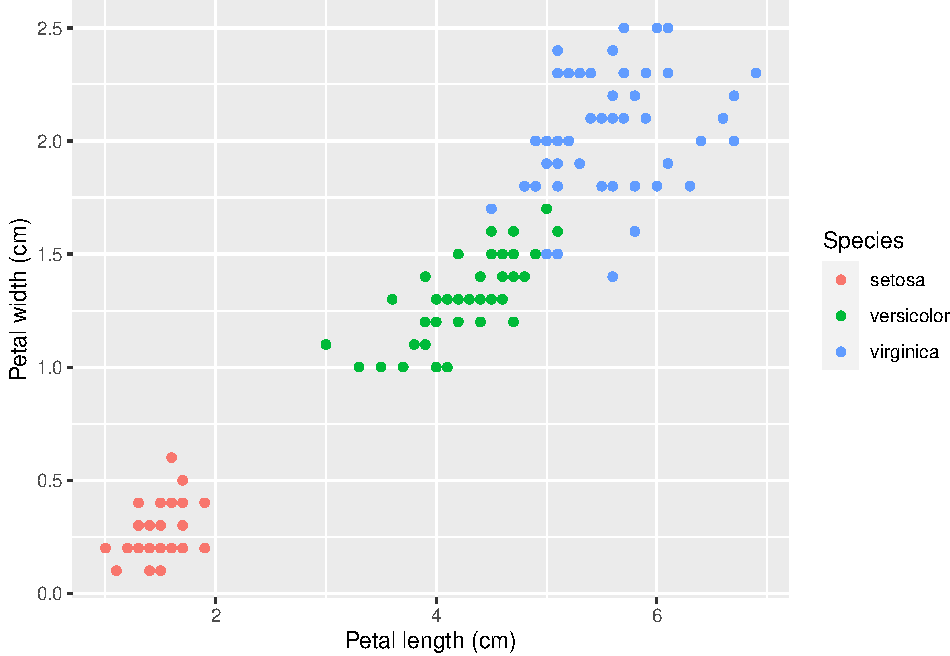
\includegraphics{s2-analysis_files/figure-latex/figure-example-1.pdf}
\caption{Petal length in irises is positively associated with petal
width. Setosas have the smallest petals, while those of versicolors and
virginicas are larger.}
\end{figure}

More information about including tables and figures in your Rmarkdown
document can be found here:
\url{https://rmd4sci.njtierney.com/figures-tables-captions-.html}.

(Don't worry if the tables or figures appear in a different place in the
PDF than they do in the Rmd file. Tables and figures might ``float''
around a little, based on what the typesetting algorithm thinks looks
best, and this is to be expected.)

\end{document}
